\subsection{Editing documentation}
In the organization, there are many activities which require a set of
document to be written and edited during the normal flow of the business.
For this reason the Information System provides a set of features, whose
aim is to build a service of documents storage.

Authenticated users are allowed to interact with the various resources
within the limits of their privileges. The task of the system, in case of
editing, is to notify that the resource is in a editing state and generate
a copy of the document in a format usable by the user.

The sequence diagram in figure \ref{3img:[sequence]editing} shows the
details of this operation.

\begin{figure}[H]
\begin{centering}
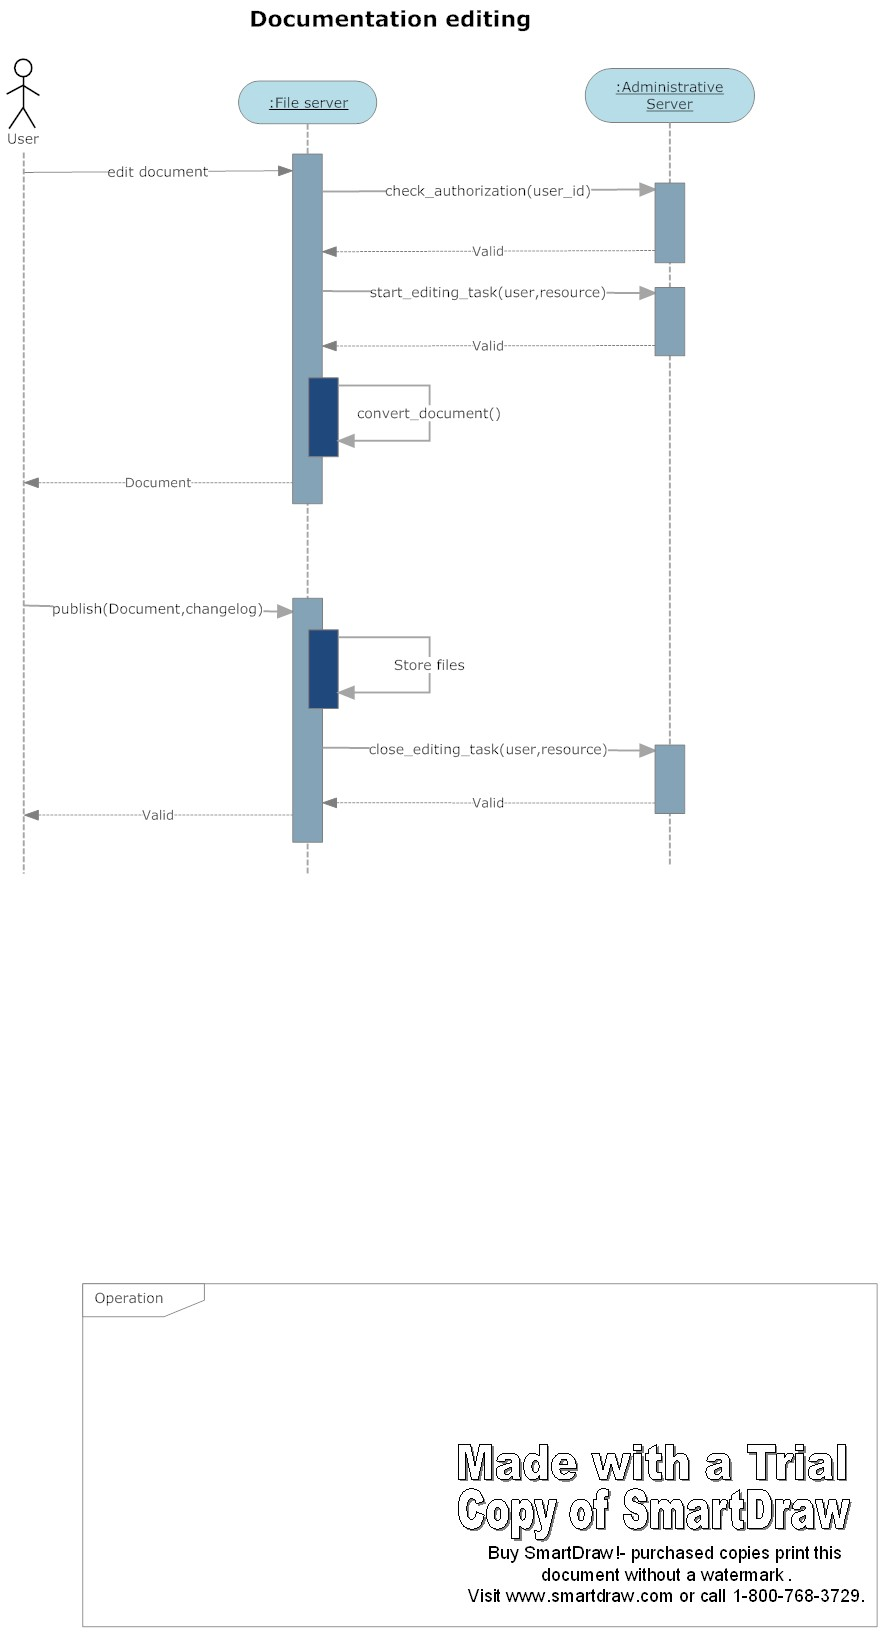
\includegraphics[scale=0.45]{assign3/sdraw/imgs/editing.jpg}
\caption{Editing documentation sequence diagram.}
\label{3img:[sequence]editing}
\end{centering}
\end{figure}
